\documentclass[conference]{IEEEtran}

%\usepackage{bookmark}

%when error about empty item in bibliography
%\makeatletter
%\def\endthebibliography{%
  %\def\@noitemerr{\@latex@warning{Empty `thebibliography' environment}}%
  %\endlist
%}
%\makeatother



% *** CITATION PACKAGES ***
%
\usepackage{cite}
%\nocite{*}

% *** GRAPHICS RELATED PACKAGES ***
%
\ifCLASSINFOpdf
   \usepackage[pdftex]{graphicx}
  % declare the path(s) where your graphic files are
   \graphicspath{{./pictures/}}
  % and their extensions so you won't have to specify these with
  % every instance of \includegraphics
  \DeclareGraphicsExtensions{.pdf,.jpeg,.png}
\else
  
\fi

\usepackage[utf8]{inputenc}


% *** MATH PACKAGES ***
%
\usepackage{amsmath}

% *** ALIGNMENT PACKAGES ***
%
\usepackage{array}

% *** PDF, URL AND HYPERLINK PACKAGES ***
%
\usepackage{hyperref}
\usepackage{url}

% correct bad hyphenation here
\hyphenation{op-tical net-works semi-conduc-tor}

\newcommand{\af}{\textsc{AF3 }}
\newcommand{\autof}{\textsc{AutoFOCUS 3 }}
\newcommand{\asp}{\textit{aspects }}
\newcommand{\cbc}{{Categorization-based concept }}
\newcommand{\cc}{\textsc{CBC }}

\usepackage{ifthen}
\usepackage{amssymb} 
\newboolean{showcomments}  
\setboolean{showcomments}{true} % toggle to show or hide comments
\ifthenelse{\boolean{showcomments}}     
  {\newcommand{\nb}[2]{
    \fcolorbox{gray}{yellow}{\bfseries\sffamily\scriptsize#1}
    {$\blacktriangleright$#2$\blacktriangleleft$}
   }
   \newcommand{\version}{\emph{\scriptsize$-$working$-$}} 
  }
  {\newcommand{\nb}[2]{}
   \newcommand{\version}{} 
  } 

% Macros for proof-reading & corrections
\usepackage[normalem]{ulem} % for \sout  
\usepackage{xcolor} 
\newcommand\tatiana[1]{\nb{Tatiana}{\textcolor{blue}{#1}}}
\newcommand\vincent[1]{\nb{Vincent}{\textcolor{green}{#1}}}

\begin{document}

\title{Quantitative Metrics for Requirements Quality a posteriori} 

\author{
\IEEEauthorblockN{Tatiana Chuprina and Vincent Aravantinos}
\IEEEauthorblockA{Fortiss GmbH\\
Munich, Germany\\
emails: \{chuprina, aravantinos\}@fortiss.org}
}

% make the title area
\maketitle

% As a general rule, do not put math, special symbols or citations
% in the abstract
\begin{abstract}
The question of "how to measure the quality of requirements?" remains problematic due to its subjectivity.

In this paper we present various quantitative metrics for assessing the quality of requirements 
assuming a relation between requirements quality and maturity of requirements, i.e., number of changes to be done 
in requirements document. We consider the number of corrections done in a requirements document 
within the requirements engineering (RE) and implementation stages; as well as their influence on the time 
for development process.

Importantly, the proposed metrics appropriate for assessing the quality of requirements only after project completion.
Therefore, this method is a good tool for empirical studies, even though not usable to assess the attributes.
\end{abstract}

% no keywords

% For peerreview papers, this IEEEtran command inserts a page break and
% creates the second title. It will be ignored for other modes.
\IEEEpeerreviewmaketitle

\section{Introduction}
\label{sec:Intro} 

\subsection{Problem}
Measuring the quality of requirements remains problematic~\cite{Fernandez2016} due to its subjectivity.
There are only few quantitative metrics to measure the quality of requirements. 
All of them are looking at intrinsic characteristic of requirements, e.g., lack of syntactic defects 
or conformity to qualitative attributes. Such approach makes them dependable on the requirements' statement and, 
therefore, decreases an accuracy of the measurement. In other words, the clear baseline for the comparison of results 
from several separate projects is vague. Assessment of same quality characteristics within different project don't assume equality in outcoming criteria.  


\subsection{Contribution}
We present various quantitative metrics for assessing the quality of requirements assuming a relation 
between the requirements quality and corrections of the requirements done within RE and system implementation work flow. 
Comparing with existing approaches, discussed in \autoref{sec:relatedwork}, our method considers the quality of 
requirements with respect to the process, measuring the number of changes and time-consumption during RE and 
implementation phases. We consider the changes in requirements document done within 
requirements engineering and implementation stages~\cite{FARBEY:1990}, and their influence on the time 
for development process. The suggested metrics take into account a maturity of the requirements 
and reflects its leverage on the product, resulting in a number from 0 (bad) - 1 (good) for a quality assessment.  
A developed system, which has passed an acceptance test by a customer, is considered as a baseline 
for the resulting product. Importantly, the proposed metrics are usable to assess the quality of requirements 
only after project completion. 

The presented approach can be considered for empirical studies; and is in plan to employ in our study 
for doctoral thesis regarding requirements categorization approach. The requirements quality with appliance of the requirements categorization approach will be measured by the proposed metrics; afterwards, the results will be compared with an outcome of the project without the requirements categorization approach.
\section{Related Work}
\label{sec:relatedwork} 

\subsection{What does ``quality'' mean?}

Despite multiple publications about requirements quality and its assessment, 
the term ``quality'' is still subjective~\cite{Mund:2017},~\cite{Femmer:2017}. 
Industry standards~\cite{ISO/IEC/IEEE:2011} specify characteristics and criteria, 
which presumed effective for improving requirements quality, e.g, completeness, unambiguity. 
Additionally, the research community provided several types of quality definition and methods for its assessment. 
For example, Lamsweerde provides a defect-based checklist to inspect requirements for possible flaws 
and errors in ~\cite{Lamsweerde:2009}; Pohl proposes a framework defining dimensions of quality: 
the specification dimension, the representation dimension, the agreement dimension~\cite{POHL:1994}.
This approach considers such imprecise and subjective attributes as requirements adequacy or pertinence, thereby purporting uncertain assessment.
Instead of analyzing the meaning of the requirements, our method takes into account a maturity of the whole requirements artifact (RA).

%This approach purports an uncertain assessment due to impreciseness of the considered attributes, 
%such as requirements adequacy or pertinence. Instead of such level of granularity for requirements 
%consideration, our method take into account a requirements artifact (RA) in general. 

Another approach implies syntactic check of the requirements text for improving its comprehension, 
correctness, ambiguity and other akin characteristics e.g.~\cite{Ferrari:2014},~\cite{Berry:2006}.
All these metrics apply intrinsic inspection of requirements and assess qualitatively the requirements' statement. 
In contrary, our metrics provide a \textit{quantitative} analysis of a full document with the requirements.

In comparison with methods described above, activity-based quality models shift their approach from inherent properties of the requirements 
to the context of process, and propose a meta quality model~\cite{Wagner:2012},~\cite{Femmer:2015}. 
Furthermore, the "quality question" also turns to a consideration of how the requirements quality impacts the project success and the relation between 
them in scientific community~\cite{Emam:1995},~\cite{Kamata:2007}, so as among practitioners~\cite{BeattyHokanson:2014}.
In contrast to the approaches, our metrics grant a quick and lightweight method for the quality assessment considering the number of the requirements' corrections.
%our metrics grant a relative simplicity level and provide a precision with cardinal number in assessment.

%Pleiad 
A series of studies about the relation between quality and project outcomes, ~\cite{Verner:2005},~\cite{Kamata:2007},~\cite{Noorwali:2015} triggers our research to the proposed metrics. Scientific papers investigating maturity of requirements~\cite{Basili:1981},~\cite{FARBEY:1990} and their complexity~\cite{Antinyan:2016} give a base for the idea of transforming a relation between requirements quality and number of changes in requirements document into quantitative measurement, but they described the quality aspects within the ongoing process. The metrics presented in this paper consider a requirements artifact as a ``black box'' for its maturity and a process of adjusting the requirements at RE and implementation phases, in a quantitative way, once a project is over.

%Now exists a vast majority of quality definitions:
%\begin{enumerate}
	%\item in industry Standards - set of attributes such as completeness, unambiguity... [ISO/IEC/IEEE-29148];
	%\item in scientific point of view, [Lamsweerde] gives a general list of characteristics, [Pohl] proposed a framework defining dimensions of quality (• the specification dimension, • the representation dimension, the agreement dimension.);
	%\item check requirements language for lacking of errors, defects, ambiguity and possible reasons for incomprehension [];
	%\item different kind of quality models such as activity-based[10], natural-language requirements specifications[7] %(activity, stupid!)
%\end{enumerate}
%
%
%\subsection{Metrics for quality measure}
%\begin{itemize}
	%\item methodology for context-specific RE artifact quality measuring has in its base an activity-based quality model [activity, stupid!] - brief description
	%\item the mentioned attributes should be satisfied 
	%\item some researchers shift their look to product quality measurement e.g [measuring success], however 
%\end{itemize}
%
%All these metrics intend to intrinsic inspection of requirements. In contrast to them, we propose the quantitative metrics for assessment of requirements quality
\section{Metrics}
\label{sec:Solution} 

%
%\begin{figure}[H]
	%\centering
		%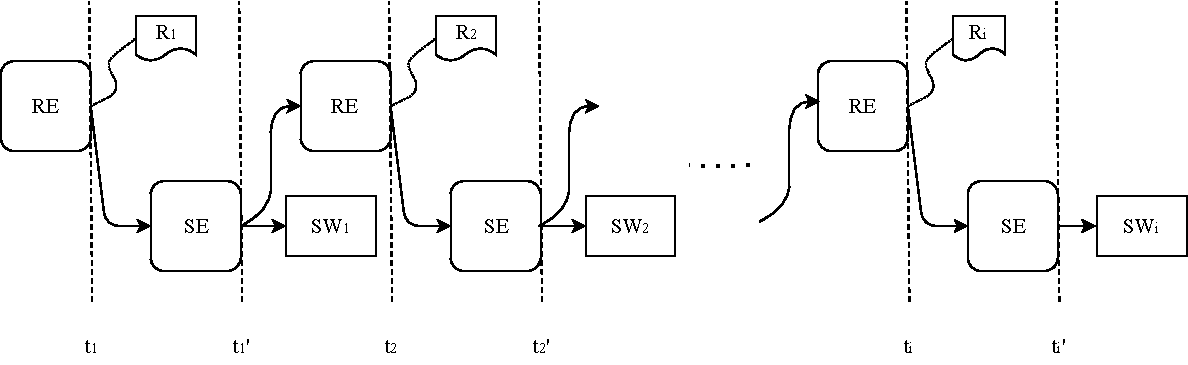
\includegraphics[width=0.8\textwidth,height=2in]{MetricsDiag.pdf}
	%\caption{Requirements engineering and development processes}
	%\label{fig:Metrics_shot}
%\end{figure}

%In these metrics we consider a maturity of requirements as a characteristic of the quality.
%
\autoref{fig:Metrics_shot} provides a graphical explanation of the metrics. The workflow is divided into requirements engineering (RE) 
and system implementation (SI) processes' iterations along the time line: $t_{1},t_{2},...,t_{m}$ - 
instants of time for RE phases (RE iteration); $t_{1}',t_{2}',...,t_{m}'$ - 
instants of time for implementation process based on the provided requirements (SI iteration).
The output of every RE iteration is RE artifact (a document with the full set of the requirements) - depicted as $R_{1},R_{2},...,R_{j}$; and every SI phase results into SI artifact, 
e.g., software architecture (shown as SW), till the end of the SI phase, which leads to the release of a product and end of the project. 

The input for the first iteration of RE process is a "raw" requirements. During the RE phase, the requirements become elaborated (changed with respect to a project's demands); the result of this process is a corrected RE artifact, that is an input 

\newpage
\hfill \break

\vspace{5.4cm}

to the next stage (SI). Therefore, we consider the initial RE artifact as a document \textit{$\mu(R_{j})=0$}. 
 
%\subsection{Metrics for a full set of requirements}

We defined, that every RE artifact has its index of maturity. The range of this metric varies from 0 to 1: 0 means ``bad'' and 1 indicates ``good'' quality.
The maturity index is inferred from a number of iterations (a certain amount of changes applied to requirements' document) and the time spent for RE and implementation process.
The more mature a requirement is, the less changes (iterations) the artifact requires, and the shorter the time for the development process. 
\textsl{Thus, the better quality of the requirements: the higher index of the requirements maturity} (\autoref{eqn:maturity_ind}). 

In \autoref{eqn:maturity_ind}, the maturity index reflects, how far the considered requirements with the certain maturity parameters (presented as a sum of the metrics for the full set of the requirements - $\sum\mu_{n}(R_{j})$) from their ``good'' state (defined as 1)

  \begin{equation}\label{eqn:maturity_ind}
\textrm{\textit{maturity index}} = \frac{1}{\sum_{i=1}^{n}\mu_{i}(R_{j})}
	\end{equation}

where $(R_{j}$) is a considered RE artifact; $j$ is an starting iteration for calculation.
%where $\mu(R_{j})$ is a calculated number of the iterations for a considered RE artifact $(R_{j}$); $j$ is an initial iteration for calculation.

Consequently, to calculate the \textit{maturity index} of the requirements, the following metrics should be determined:

 \begin{equation}\label{eqn:mu1}
\mu_{1}(R_{j}) = m-j
	\end{equation}
	
\textrm{end of the number of iterations for the requirements} $R_{j}$;

 \begin{equation}\label{eqn:mu2}
\mu_{2}(R_{j}) = t_{m}\acute{}-t_{j}    
 \end{equation}

\textrm{amount of time (in hours) between initial and the last phases of the development process applying the requirements} $R_{j}$;

%\begin{equation}\label{eqn:mu3}
%\mu_{3}(R_{j}) = \displaystyle\sum_{j} t_{j+1}-t_{j}\acute{}
%\end{equation}
%
%,\textrm{total amount of time (in hours) required for SI process};


%(here, along with requirements' maturity, we can also talk about such quality criterion as the requirements' comprehensibility);
%$\mu_{4} = \displaystyle\sum_{j} (t_{j+1}-t_{j}\acute{} + p_{j}*(t_{j}\acute{} - t_{j}))$

%\subsection{Metrics for a single requirement}



\section{Conclusion}
\label{sec:conclusion}

\tatiana{Pros:} The proposed metrics provide a uniformity in measurements of requirements quality; baseline for all assessment; Simplicity; can be used in empirical measurements.
\tatiana{Cons:}
\begin{itemize}
	\item  Firstly,  the problem of this approach is: it doesn't take into account the quality of project and its correlation with the requirements quality.
\item Secondly, the approach is theoretic (academic) and has not yet been applied on practice.
\end{itemize}
.

% no \IEEEPARstart


%\section{Conclusion}
%The conclusion goes here.

% references section

\bibliographystyle{IEEEtran}
\bibliography{RQworkshopBib}
\end{document}


